\documentclass[a4paper]{article}
\usepackage{student}
\usepackage{graphicx}
\usepackage{caption}
\usepackage[version=4]{mhchem}
\usepackage{tikz}
\usetikzlibrary{shapes.geometric, arrows.meta, positioning, decorations.pathreplacing}
\usepackage{enumitem}

\tikzstyle{arrow} = [thick,->,>=stealth]

% Definindo o estilo de destaque com linhas pontilhadas
\tikzstyle{highlight} = [draw, dashed, thick, rectangle, rounded corners, inner sep=0.2cm, orange]


\tikzstyle{startstop} = [
    rectangle, rounded corners, minimum width=0.5cm,
    text centered, draw=black, fill=blue!10, font=\small
]
\tikzstyle{startstop_S} = [
    rectangle, rounded corners, minimum width=0.5cm, minimum height=0.8cm,
    text centered, draw=black, fill=green!30, font=\small
]
\tikzstyle{decision} = [
    diamond, aspect=2, draw=black, fill=orange!15, align=center,
    text centered, inner sep=0pt, font=\small
]
\tikzstyle{decision_S} = [
    diamond, aspect=2, draw=black, fill=orange!30, align=center,
    text centered, inner sep=0pt, font=\small
]
\tikzstyle{arrow} = [thick,->,>=stealth]



% Metadata
\date{\today}
\setmodule{PGF5261/IFUSP: Teoria de Grupos Aplicada a Sólidos e Moléculas. Prof.: Lucy Assali} 
\setterm{1o. semestre, 2025}

%-------------------------------%
% Other details
% TODO: Fill these
%-------------------------------%
\title{Exercício 01 - 28/03}
\setmembername{Nara Avila Moraes}  % Fill group member names
\setmemberuid{5716734}  % Fill group member uids (same order)

%-------------------------------%
% Add / Delete commands and packages
% TODO: Add / Delete here as you need
%-------------------------------%
\usepackage{amsmath,amssymb,bm}

\newcommand{\KL}{\mathrm{KL}}
\newcommand{\R}{\mathbb{R}}
\newcommand{\E}{\mathbb{E}}
\newcommand{\T}{\top}

\newcommand{\expdist}[2]{%
        \normalfont{\textsc{Exp}}(#1, #2)%
    }
\newcommand{\expparam}{\bm \lambda}
\newcommand{\Expparam}{\bm \Lambda}
\newcommand{\natparam}{\bm \eta}
\newcommand{\Natparam}{\bm H}
\newcommand{\sufstat}{\bm u}

% Main document
\begin{document}
    % Add header
    \header{}

\textbf{Questão 1.}
Considere as simetrias da molécula de amônio \ce{NH3} e responda os seguintes ítems:

\begin{center}
\begin{minipage}{0.4\textwidth}
    \centering
     \includegraphics[width=0.4\textwidth]{figuras/amonio.png}
        \captionof{figure}{Molécula de Amônio}
\end{minipage}
\hfill
\begin{minipage}{0.55\textwidth}
    \begin{itemize}
      \item[(1.1)] Identifique o \textbf{grupo} de simetria da molécula.
      \item[(1.2)] Qual é a \textbf{ordem} desse grupo?
      \item[(1.3)] Apresente a \textbf{tabela de multiplicação}.
      \item[(1.4)] Esse grupo é \textbf{cíclico}? Justifique.
      \item[(1.5)] O grupo é \textbf{abeliano}? Justifique.
      \item[(1.6)] Quais são as \textbf{classes} desse grupo?
    \end{itemize}
\end{minipage}
\end{center}


    % Use `answer` environment to add solutions
    % \begin{answer}[Question 1.1] for example starts an environment formatted
    % for Question 1.1

    \begin{answer}[Ítem 1.1 - Grupo]
\begin{center}
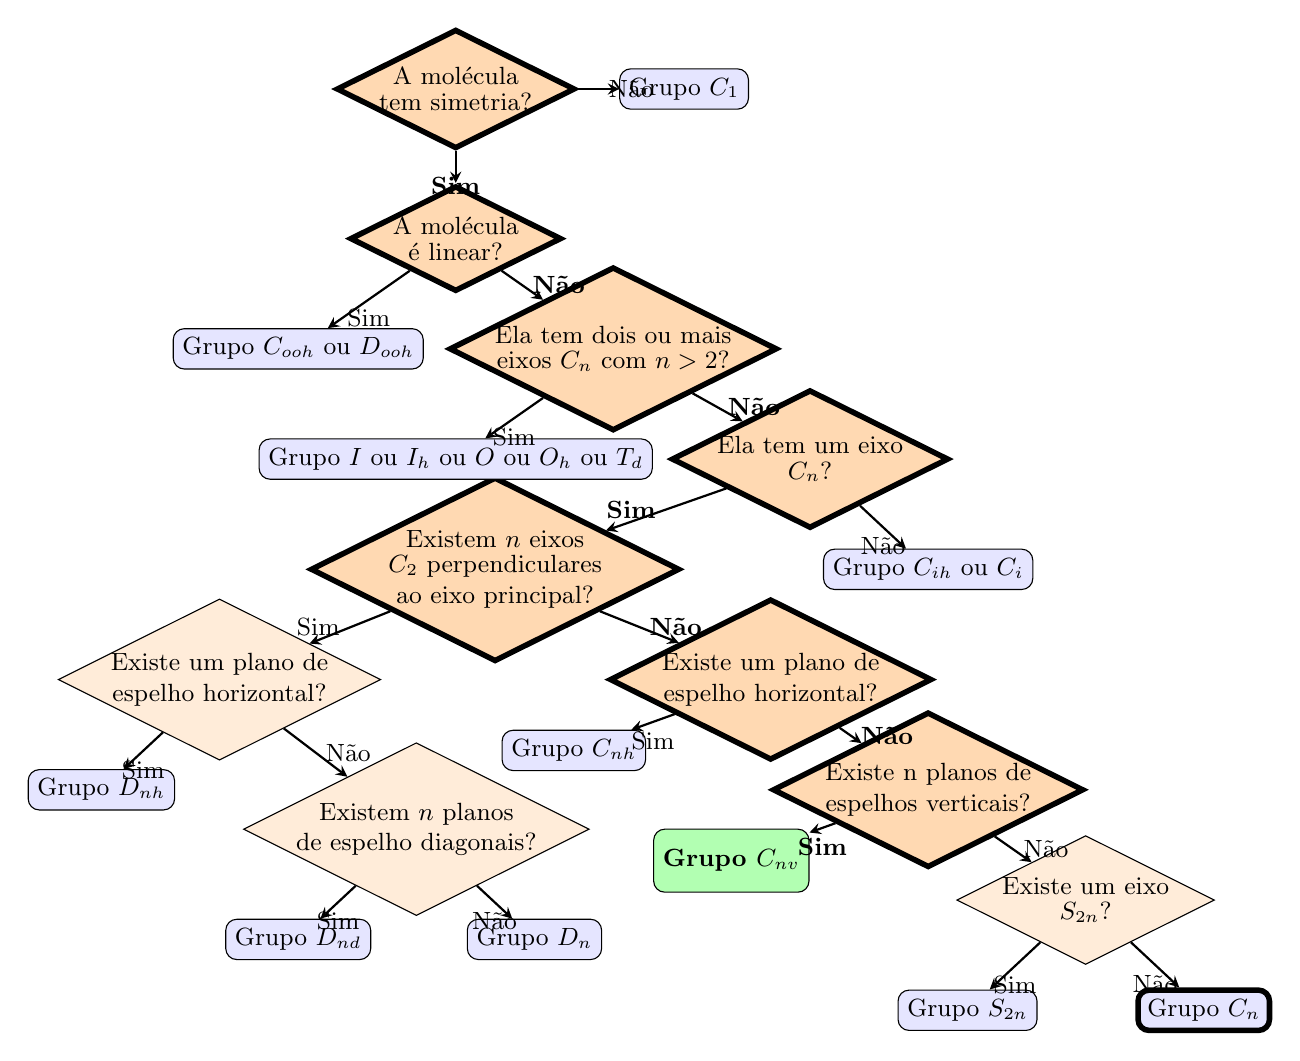
\begin{tikzpicture}[node distance=1.4cm]
% Definindo as 15 decisões
\node (Q_1) [decision_S, xshift=-7cm, line width=0.7mm] {\shortstack{A molécula\\tem simetria?}};
\node (Q_2) [decision_S, below of=Q_1, yshift=-0.5cm, line width=0.7mm] {\shortstack{A molécula\\é linear?}};
\node (Q_4) [decision_S, below of=Q_2, xshift=2cm, line width=0.7mm] {\shortstack{Ela tem dois ou mais\\eixos \( C_n \) com \( n>2 \)?}};
\node (Q_6) [decision_S, below of=Q_4, xshift=2.5cm, line width=0.7mm] {\shortstack{Ela tem um eixo\\\( C_n \)?}};
\node (Q_9) [decision_S, below of=Q_6, xshift=-4cm, line width=0.7mm] {\shortstack{Existem \( n \) eixos\\\( C_2 \) perpendiculares\\ao eixo principal?}};
\node (Q_10) [decision, below of=Q_9, xshift=-3.5cm] {\shortstack{Existe um plano de\\espelho horizontal?}};
\node (Q_11) [decision, below of=Q_10, xshift=2.5cm, yshift=-0.5cm] {\shortstack{Existem \( n \) planos\\de espelho diagonais?}};
\node (Q_12) [decision_S, below of=Q_9, xshift=3.5cm, line width=0.7mm] {\shortstack{Existe um plano de\\espelho horizontal?}};
\node (Q_13) [decision_S, below of=Q_12, xshift=2cm, line width=0.7mm] {\shortstack{Existe n planos de\\espelhos verticais?}};
\node (Q_14) [decision, below of=Q_13, xshift=2cm] {\shortstack{Existe um eixo\\\( S_{2n} \)?}};

% Caminhos
\node (CooDoo) [startstop, below of=Q_2, xshift=-2cm] {Grupo $C_{ooh}$ ou $D_{ooh}$};
\node (G_alta_simetria) [startstop, below of=Q_4, xshift=-2cm] {Grupo $I$ ou $I_h$ ou $O$ ou $O_h$ ou $T_d$};
\node (G_baixa_simetria) [startstop, below of=Q_6, xshift=1.5cm] {Grupo $C_{ih}$ ou $C_i$};
\node (Dnh) [startstop, below of=Q_10, xshift=-1.5cm] {Grupo $D_{nh}$};
\node (Dnd) [startstop, below of=Q_11, xshift=-1.5cm] {Grupo $D_{nd}$};
\node (Dn) [startstop, below of=Q_11, xshift=1.5cm] {Grupo $D_n$};
\node (Cnv) [startstop_S, below of=Q_13, xshift=-2.5cm, yshift=0.5cm] {\textbf{Grupo $C_{nv}$}};
\node (Cnh) [startstop, below of=Q_12, xshift=-2.5cm, yshift=0.5cm] {Grupo $C_{nh}$};
\node (S2n) [startstop, below of=Q_14, xshift=-1.5cm] {Grupo $S_{2n}$};
\node (Cn) [startstop, below of=Q_14, xshift=1.5cm, line width=0.7mm] {Grupo $C_n$};
\node (C1) [startstop, right of=Q_1, xshift=1.5cm] {Grupo $C_1$};

% Connections
\draw [arrow] (Q_1) -- node[anchor=north, font=\small] {\textbf{Sim}} (Q_2);
\draw [arrow] (Q_2) -- node[anchor=west, font=\small] {\textbf{Não}} (Q_4);
\draw [arrow] (Q_4) -- node[anchor=west, font=\small] {\textbf{Não}} (Q_6);
\draw [arrow] (Q_6) -- node[anchor=east, font=\small] {\textbf{Sim}} (Q_9);
\draw [arrow] (Q_9) -- node[anchor=east, font=\small] {Sim} (Q_10);
\draw [arrow] (Q_10) -- node[anchor=west, font=\small] {Não} (Q_11);
\draw [arrow] (Q_9) -- node[anchor=west, font=\small] {\textbf{Não}} (Q_12);
\draw [arrow] (Q_12) -- node[anchor=west, font=\small] {\textbf{Não}} (Q_13);
\draw [arrow] (Q_13) -- node[anchor=west, font=\small] {Não} (Q_14);

% Final Connections
\draw [arrow] (Q_2) -- node[anchor=north, font=\small] {Sim} (CooDoo);
\draw [arrow] (Q_4) -- node[anchor=north, font=\small] {Sim} (G_alta_simetria);
\draw [arrow] (Q_6) -- node[anchor=north, font=\small] {Não} (G_baixa_simetria);
\draw [arrow] (Q_10) -- node[anchor=north, font=\small] {Sim} (Dnh);
\draw [arrow] (Q_11) -- node[anchor=north, font=\small] {Sim} (Dnd);
\draw [arrow] (Q_11) -- node[anchor=north, font=\small] {Não} (Dn);
\draw [arrow] (Q_12) -- node[anchor=north, font=\small] {Sim} (Cnh);
\draw [arrow] (Q_13) -- node[anchor=north, font=\small] {\textbf{Sim}} (Cnv);
\draw [arrow] (Q_14) -- node[anchor=north, font=\small] {Sim} (S2n);
\draw [arrow] (Q_14) -- node[anchor=north, font=\small] {Não} (Cn);
\draw [arrow] (Q_1) -- node[anchor=west, font=\small] {Não} (C1);

\end{tikzpicture}
\end{center}
Conforme ilustrado na \textbf{Figura 1}, a molécula de \( \mathrm{NH}_3 \) possui:
\begin{itemize}[noitemsep, topsep=0pt, label=--]
    \item Um eixo de rotação (\({C_n}\)) passando pelo átomo de nitrogênio e o centro do triângulo formado pelos hidrogênios "da base", com simetria de rotação de 120\textdegree  (\( C_3 \));
    \item Três planos de reflexão verticais, que contêm o eixo \( C_3 \), (\( \sigma_v \)) que passa por cada hidrogênio e segue pela bisetriz do angulo $\hat{O}_{HH}$ do triângulo da base referido acima, com também 120\textdegree entre eles.
\end{itemize}
De acordo com as simetrias citadas e conforme ilustrado pelo fluxograma o grupo de simetria da molécula de amônia é o \( C_{3v} \):
    \end{answer}
    
    \begin{answer}[Ítem 1.2 - Ordem]A ordem de um grupo é o número total de elementos de simetria. O grupo \( C_{3v} \) contém:
\begin{itemize}
  \item 1 identidade (\( E \));
  \item 2 rotações: \( C_3 \) e \( C_3^2 \), 120\textdegree e 240\textdegree;
  \item 3 reflexões em planos verticais que passam por \(H_{1}\) - \(N\), \(H_{2}\) - \(N\) e \(H_{3}\) - \(N\) (\( \sigma_v, \sigma_v', \sigma_v'' \)).
\end{itemize}

Logo, a ordem do grupo é \( 6 \). \[
  \{E, C_3, C_3^2, \sigma_v, \sigma_v', \sigma_v''\}
  \]
    \end{answer}

        \begin{answer}[Ítem 1.3 - Tabela de Multiplicação]
    Aplicando as operações duas a duas entre os elementos do grupo de simetria, obtemos todas as 36 combinações possíveis. Em cada caso, a operação resultante também pertence ao grupo, o que evidencia a propriedade de fechamento, uma das exigências fundamentais para a definição de grupo. A tabela de multiplicação do grupo \( C_{3v} \) resultante abaixo foi obtida aplicando a operação dos elementos da linha como operadores aplicados à esquerda, ou seja primeiro e os operadores da coluna depois ( \(M_{ij} = g_i \circ g_j\), onde \( g_i \) é o primeiro elemento da \textbf{linha} \( i \) e \( g_j \) é o primeiro elemento da \textbf{coluna}) \( j \), já que essa operação não necessariamente comuta:

\textbf{Tabela de multiplicação resultante:}

  \[
  \begin{array}{c|cccccc}
    \cdot & E & C_3 & C_3^2 & \sigma_v & \sigma_v' & \sigma_v'' \\
    \hline
    E & E & C_3 & C_3^2 & \sigma_v & \sigma_v' & \sigma_v'' \\
    C_3 & C_3 & C_3^2 & E & \sigma_v' & \sigma_v'' & \sigma_v \\
    C_3^2 & C_3^2 & E & C_3 & \sigma_v'' & \sigma_v & \sigma_v' \\
    \sigma_v & \sigma_v & \sigma_v'' & \sigma_v' & E & C_3 & C_3^2 \\
    \sigma_v' & \sigma_v' & \sigma_v & \sigma_v'' & C_3^2 & E & C_3 \\
    \sigma_v'' & \sigma_v'' & \sigma_v' & \sigma_v & C_3 & C_3^2 & E \\
  \end{array}
  \]
        
    \end{answer}

    \begin{answer}[Ítem 1.4 - Cíclico]
    Um grupo cíclico é gerado por potências de um único elemento. Para o grupo \( C_{3v} \), os elementos de reflexão não podem ser gerados a partir das potências de \( C_3 \). Portanto, o grupo não é cíclico.
    \end{answer}

        \begin{answer}[Ítem 1.5 - Abeliano]
   O grupo \( C_{3v} \) não é abeliano, pois a ordem da composição importa, ou seja, este grupo não tem a propriedade adicional de comutatividade. Por exemplo, \( C_3 \cdot \sigma_v \neq \sigma_v \cdot C_3 \). Observando a tabela de multiplicação, caso o grupo fosse abeliano teriamos uma simetria em relação à diagonal, que seria composta apenas de transformações/elemento E, o que não é o caso.
    \end{answer}

        \begin{answer}[Ítem 1.6 - Classes]
    As classes sumarizam as simetrias do grupo, agrupando operações diferentes mas que são fisicamente equivalentes, e que podem nos ajudar a reduzir o problema estudado permitindo uma resposta unica do problema para cada classes de simetrias. As classes de conjugação do grupo \( C_{3v} \) são:
  \[
  \{E\}, \quad \{C_3, C_3^2\}, \quad \{\sigma_v, \sigma_v', \sigma_v''\} \]
    \end{answer}
\end{document}

        \begin{figure}
            \includegraphics[width=0.5\linewidth]{figuras/Molecula_amonio.png}
            \caption{Molécula de Amônio}
            \label{fig:enter-label}
        \end{figure}